The Finite Element Method (FEM) is used for finding approximate solutions of partial
differential equations. It is based on an expansion of the dependent variable(s), the
particle flux in our case, into a linear combination of polynomial trial functions defined
over subvolumes. The trial functions space must be chosen so as to ensure that improvement in the numerical approximation occurs with increase in the number I of subvolumes and/or
with the degree K of the polynomial trial functions. The trial functions are known a priori and the corresponding coefficients can be found using a weighted residual approach or a variational formulation. In this section, We have chosen to present the variational formulation, as it brings two important benefits:
\begin{enumerate}
    \item The intrinsic symmetry of the one-speed diffusion equation is always preserved by
the discretization process,
    \item The boundary conditions are introduced in a consistent way.
\end{enumerate} 

\begin{figure}[h!]
    \centering
    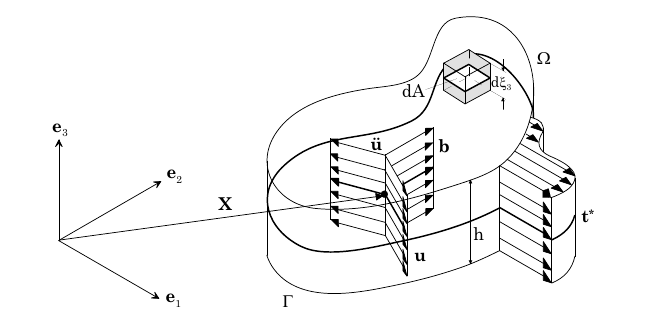
\includegraphics[scale=0.6]{Figures/Chapter2/planeElement.png}
    \decoRule   
    \caption{Representation of the three-dimensional continuum in plane elements}
    \label{fig:plane-element}
\end{figure}
\noindent
The FEM can be applied to various types and form of subvolumes or elements. In the following section first the basic equations of plane finite elements are derived from the
consideration of the three-dimensional continuum with the insertion of the fundamental assumptions of planar continua. Afterwards, plane elements are classified according to the element form and the order of the shape functions and the discretization of planar continua is explained in
details with the help of the four-node, linear, isoparametric Lagrange element. Furthermore,
retangular elements of higher approximation order and are discussed.
%--------
\subsection{Mechanical Problem}
\label{planeproblem}
In this section, we will discuss  two popular problems of the plane element: plane stress and plane strain
\begin{figure}[H]
    \centering
    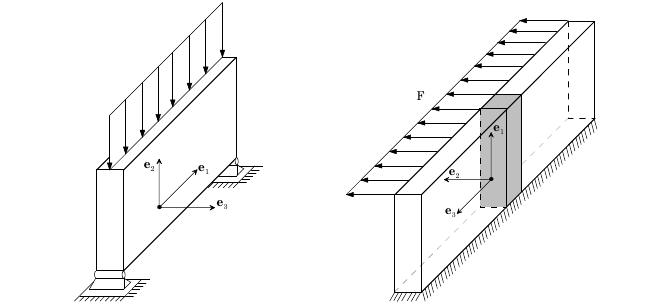
\includegraphics[scale=0.5]{Figures/Chapter2/110.png}
    \decoRule   
    \caption{ Examples for the application of plane stress and strain states}
    \label{fig:110}
\end{figure}
%-----plane strain stress
\vspace{0.38cm} \textbf{a) \textit{Plane Stress State}} \\
A representative plane element is examined, which lies in the plane spanned by the base vectors
$e_1$ and $e_2$ . In the case of a plane stress state it is assumed that the stress components $\sigma_{33}$ , $\sigma_{13}$ and $\sigma_{23}$ vanish

\begin{equation}
\begin{gathered}
  \sigma_{11}=\sigma_{22}=\sigma_{33}=0 \\
    \varepsilon_{13}=\varepsilon_{23}=0
\end{gathered}
\end{equation}
with the remaining stress components being constant in the direction of the base vector $e_3$ , see Fig. \ref{fig:111}
\begin{figure}[H]
    \centering
    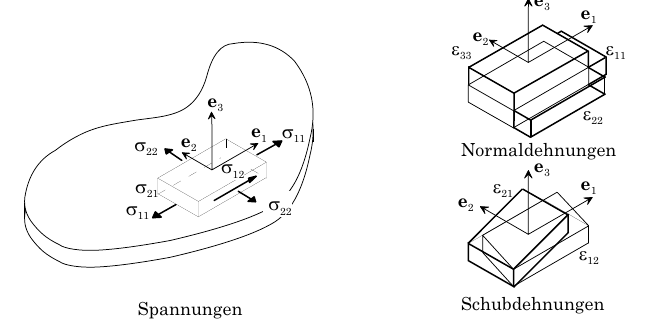
\includegraphics[scale=0.5]{Figures/Chapter2/111.png}
    \decoRule   
    \caption{Plane stress state}
    \label{fig:111}
\end{figure}
%-----plane strain stress
\vspace{0.38cm} \textbf{b) \textit{Plane Strain State}} \\
Again, a representative plane element is examined which lies in the plane spanned by the base
vectors $e_1$ and $e_2$ , see Fig.\ref{fig:112}. For the generation of the plane strain state it is assumed that the strain components $ \varepsilon_{33} , \varepsilon_{13}$ and $\varepsilon_{23} $vanish. the stress components $\sigma_{23} , \sigma_{13}$ become zero; the stress $\sigma_{33}$ , on the contrary, is different from zero.
\begin{equation}
\begin{gathered}
  \varepsilon_{11}=\varepsilon_{22}=\varepsilon_{33}=0 \\
    \sigma_{13}=\sigma_{23}=0
\end{gathered}
\end{equation}
\begin{figure}[H]
    \centering
    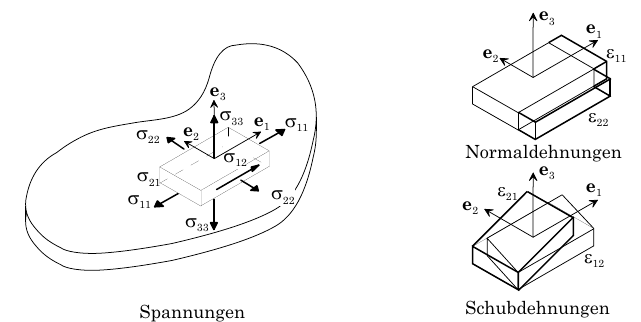
\includegraphics[scale=0.5]{Figures/Chapter2/112.png}
    \decoRule   
    \caption{  Plane strain state}
    \label{fig:112}
\end{figure}
%-------------------------------------------

%-----plane strain stress
\subsection{Geometry}
A planar structure, or a two-dimensional continuum, is generated by the degeneration of the
three-dimensional continuum onto a middle surface A and the thickness h. Due to this reason,
the properties of the three-dimensional continuum are represented by the properties of the
middle surface within the context of the modelling of a plane finite element (see Fig. \ref{fig:plane-element}).
Two-dimensional elements of structural mechanics are
\begin{itemize}
    \item Plane elements which are characterized by a small thickness $h$ relative to the dimensions of the middle surface and are characterized by the plane stress state ( see section \ref{planeproblem})
    
    \item Plane elements which describe an infinite dimension of the mechanical problem in $e _3$ - direction and are, thus, described by the plane strain state ( see section \ref{planeproblem}) 
\end{itemize}
\noindent
The thickness $h$ represents in the case of plane strain state the infinite thickness or the unit
thickness; therefore the thickness of finite elements of the plane strain state is often given the
value one. Within the context of this lecture the element thickness must be considered a parameter also for the plane strain state in order to guarantee a generalized description of elements of
the plane stress and strain state.
The geometrical description of such a two-dimensional element follows from the position vector
of a material point on the middle surface
\begin{equation}
    {\bf X}=[X_1 \quad X_2]^T
\end{equation}
and its motion when a load is applied.

%------------------------------------------------------------------------------------
%------------------------------------------------------------------------------------

\subsection{Kinetics}
The first fundamental assumption for the realization of the degeneration of the three- dimensional continuum to the two-dimensional continuum is the assumption of the stress and strain
state, where it is distinguished between the plane stress state (ES) and the plane strain state
(EV).
\begin{equation}
\label{eqn:3.2}
    \begin{gathered}
ES:{\sigma _{33}} = {\sigma _{23}} = {\sigma _{13}} = 0\\
EV:{\sigma _{33}} = \nu \left( {{\sigma _{11}} + {\sigma _{22}}} \right),{\sigma _{23}} = {\sigma _{13}} = 0
\end{gathered}
\end{equation}
When the plane stress state is assumed to hold the internal kinetics is uniquely described by
the components $\sigma_{11}$ , $\sigma_{22}$ and $\sigma_{12}$ (see Fig.1.11). In the case of plane strain state additionally
the normal stress component $\sigma_{33}$is present (see Fig. 1.12). For a complete and unique
characterization of the stress state this normal component of the stress tensor is actually not
necessary, as it can be computed directly from the stress components $\sigma_{11}$ and $\sigma_{22}$ according to
Eq. (1.74). For the formulation of the internal virtual work the component $\sigma_{33}$ is also of no
significance, for the conjugated strain component $\varepsilon_{33}$ is zero according to the assumptions of
the plane strain state. Therefore, it is enough, both for the plane stress state and for the plane
strain state, to define the stress vector
\begin{equation}
\label{eqn:3.3}
    \sigma=[\sigma_{11} \quad \sigma_{22} \quad \sigma_{33}]^T
\end{equation}

With three components for the formulation of the internal virtual work and, thus, also for the
generation of the discretized stiffness relation of plane finite elements. In accordance woth
the above-mentioned kinetic assumptions the volulme loads $b_3$ and the Neumann boundary
conditions $t^{*}_3$ vanish in the $e_3$-direction, wherefrom also the corresponding vectors are described
by two components each (see Fig. \ref{fig:110}).
\begin{equation}
\label{eqn:3.4}
 \boldsymbol{b}=\left[\begin{array}{ll}b_{1} & b_{2}\end{array}\right]^{T} \qquad \qquad \boldsymbol{t}^{\star}=\left[\begin{array}{ll}t_{1}^{\star} & t_{2}^{\star}\end{array}\right]^{T} 
\end{equation}

%----------------------------------------
\subsection{Kinematics}
The second fundamental assumption of plane finite elements concerns the displacement field:
all material points at the normal of the middle surface exhibit under deformation the same
displacements in the directions $e_1$ and $e_2$ .
\begin{equation}
\label{eqn:3.5}
 u_{1}=u_{1}\left(X_{1}, X_{2}\right) \qquad \qquad u_{2}=u_{2}\left(X_{1}, X_{2}\right) 
 \label{eqn:3.5}
\end{equation}

The displacement component $u_3$ is zero in the case of plane strain state. For the plane stress
state $u_ 3$ is different from zero. However, it follows from the assumptions for the volume and surface loads in Eq. (\ref{eqn:3.4}) that this displacement component has no contribution to the virtual
work of the external loads. Here, it is assumed without a proof 1 that also the portion of this component in the virtual wotk of the inertial forces vanishes during deformation. Thus, the
deformation of the degenerated two-dimensional continuum can be described uniquely by the displacement vector
\begin{equation}
 \boldsymbol{u}\left(X_{1}, X_{2}\right)=\boldsymbol{u}(\boldsymbol{X})=\left[\begin{array}{ll}u_{1}\left(X_{1}, X_{2}\right) & u_{2}\left(X_{1}, X_{2}\right)\end{array}\right]^{T} 
 \label{eqn:3.6}
\end{equation}
expressed, according to Eq. (\ref{eqn:3.5}), only in terms of the coordinates of the plane spanned by the
basis vectors e 1 and e 2 . From this follow directly the variation of the displacement vector and,
by twice differentiating Eq. (\ref{eqn:3.6}) with respect to time, the acceleration vector.
\begin{equation}
\label{eqn:3.7}
 \delta \boldsymbol{u}(\boldsymbol{X})=\left[\delta u_{1}\left(X_{1}, X_{2}\right) \quad \delta u_{2}\left(X_{1}, X_{2}\right)\right]^{T} \qquad \ddot{\boldsymbol{u}}(\boldsymbol{X})=\left[\begin{array}{ll}\ddot{u}_{1}\left(X_{1}, X_{2}\right) & \ddot{u}_{2}\left(X_{1}, X_{2}\right)\end{array}\right]^{T} 
\end{equation}

The complete description of the degenerated two-dimensional continuum requires furthermore the formulation of the Dirichlet boundary conditions
\begin{equation}
\label{eqn:3.8}
 \boldsymbol{u}(\boldsymbol{X}, t)=\boldsymbol{u}^{\star}(\boldsymbol{X}, t\qquad \qquad \forall \quad \boldsymbol{X} \in \Gamma_{u} 
\end{equation}
and the initial conditions of the displacement vector and the acceleration vector, where it should
be noted that only one of the two initial conditions has to be prescribed, as the second one results
from the evaluation of the equation of motion of the degenerated continuum at time $t = 0$
\begin{equation}
\label{eqn:3.9}
 \begin{aligned} \boldsymbol{u}(\boldsymbol{X}, t=0) &=\boldsymbol{u}^{\star}(\boldsymbol{X}) & \qquad \forall \quad \boldsymbol{X} \in \Omega \\ \ddot{\boldsymbol{u}}(\boldsymbol{X}, t=0) &=\ddot{\boldsymbol{u}}^{\star}(\boldsymbol{X}) & & \end{aligned} 
\end{equation}

It remains to describe the strain state of the degenerated continuum by the strain vector $\varepsilon$. In
accordance with the already discussed assumptions of plane stress or plane strain states this
vector can be obtained by the assembly of the strain components$\varepsilon_{ 11 }$, $\varepsilon_ {22}$ and $2\varepsilon_ {12}$ alone.
\begin{equation}
\label{eqn:3.10}
 \varepsilon=\left[\begin{array}{lll}\varepsilon_{11} & \varepsilon_{22} & 2 \varepsilon_{12}\end{array}\right]^{T} 
\end{equation}

The component $\varepsilon_{ 33 }$that is different from zero in the plane stress state is not needed for the unique characterization of the strain state, for this strain component can be combined linearly with the components $\varepsilon_{ 11}$ and $\varepsilon_{ 22}$ . In addition, the same argumentation
for the vanishing virtual work of the strain component $\varepsilon_{ 33}$ as in the definition of the stress vector
$\sigma$, applies here. The strain tensor can be computed in tensor notation
\begin{equation}
\label{eqn:3.11}
 \varepsilon=\nabla^{\mathrm{sym}} \boldsymbol{u} \qquad \qquad \varepsilon_{\alpha \beta}=\frac{1}{2}\left(u_{\alpha, \beta}+u_{\beta, \alpha}\right) 
\end{equation}
where it should be considered that the indices $\alpha$ and $\beta$ can take only the values one or two due to the degeneration ($\alpha$, $\beta$ = 1, 2). Besides, the strain vector can be obtained by application of the differential operator $D_\varepsilon$ to the displacement vector $u$.
\begin{equation}
\label{eqn:3.12}
 \varepsilon=\mathbf{D}_{\varepsilon} u \qquad \qquad
 \left[\begin{array}{c}\varepsilon_{11} \\ \varepsilon_{22} \\ 2 \varepsilon_{12}\end{array}\right]=\left[\begin{array}{cc}\frac{\partial}{\partial X_{1}} & 0 \\ 0 & \frac{\partial}{\partial X_{2}} \\ \frac{\partial}{\partial X_{2}} & \frac{\partial}{\partial X_{1}}\end{array}\right]\left[\begin{array}{l}u_{1} \\ u_{2}\end{array}\right] 
\end{equation}
Thus, it follows directly from the Eqs. (\ref{eqn:3.5}) that the components of the strain vector $\varepsilon_{\alpha \beta}$ are constant along the thickness of the degenerated continuum.

\begin{equation}
\label{eqn:3.13}
 \varepsilon=\varepsilon\left(X_{1}, X_{2}\right) 
\end{equation}
%----------------------------------------
\subsection{Finite Element Discretization}
The finite element discretization and analysis of plane continua consists of the partitioning of
the structure, or the domain under consideration, into finite elements and the approximation
of continuously distributed physical quantities (e.g. displacements) by discrete nodal degrees
of freedom and the assumption of their distribution over the element area. This assumption is
associated with the choice of shape functions, which depend on the variables $\varepsilon_1$ and $\varepsilon_2$ for the case of plane elements.

In contrast to the spatial truss frame, for which a constructively discrete structure was available
already before the mathematical discretization, now a two-dimensional continuum $\Omega$ must be
subdivided into finite subdomains $\Omega^e$ .
\begin{equation}
\label{eqn:3.28}
\begin{gathered}
    \Omega  = \bigcup\limits_{e = 1}^{NE} {{\Omega ^e}}\\
    with \quad {\Omega ^i} \cap {\Omega ^j} = \emptyset {\rm{ }} \quad for \quad i \ne 
\end{gathered}
\end{equation}

Inside these finite subdomains $\Omega^e$ , or finite elements $e$, the continuous field variables are approximated by means of shape functions and discrete nodal degrees of freedom. A basis for the
development of plane finite elements is the requirement that the principle of virtual work should
be fulfilled for every finite element $e$. 
\begin{equation}
\label{eqn:3.29}
 \delta W_{\mathrm{dyn}}^{e}+\delta W_{\mathrm{int}}^{e}=\delta W_{\mathrm{ext}}^{e} 
\end{equation}
The topological element structure, formed by the subdivision into subdomains $\Omega^e$ , is called finite element mesh and the process of its generation is meshing or mesh generation.

Accuracy of the finite element analysis increases with increasing the polynomial degree $p$, for which
reason the basic elements (3- or 4-node elements) are often substituted by elements of higher
polynomial degree. Furthermore, higher-order elements are essentially more suitable than the basic elements for discretizing domains $\Omega$ with curved boundaries, due to the possibility to
describe curved element boundaries. As is to be expected from the previous discussions, \textsc{Lagrange} elements with an internal node provide more accurate results than serendipity elements
without an internal node. The difference in the accuracy is, however, negligible and cannot level
out the shortcoming of the additionally needed internal degrees of freedom of the Lagrange
element (which are of importance particularly by the assembled system). As a disadvantage of
serendipity elements, it should be added that they are restricted to a polynomial degree $p < 4$

\subsection{Shape Functions of Plane Elements }
Within the framework of development of plane finite elements, shape functions of the varying
natural coordinates $\xi_1$ and $ \xi_2$ are used. These shape functions represent polynomials in the
two-dimensional space of the form


\begin{figure}
    \centering
    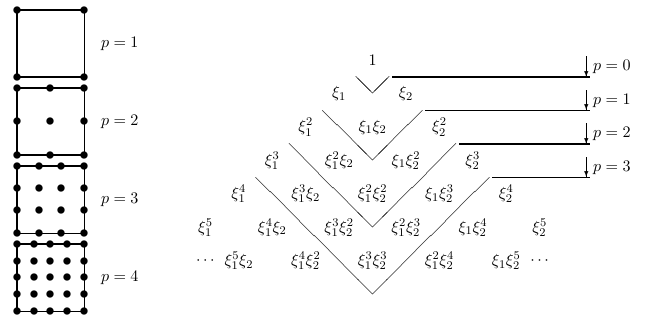
\includegraphics[scale=0.5]{Figures/Chapter2/LagrangePascal.png}
    \caption{Two-dimensional Lagrange ansatz polynomials of quadrangular elements in the
 \textsc{Pascal} triangle  }
    \label{fig:3.5}
\end{figure}


\begin{figure}
    \centering
    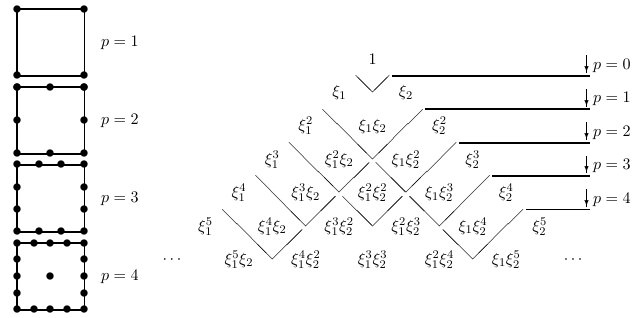
\includegraphics[scale=0.5]{Figures/Chapter2/polynomialsPascal.png}
    \caption{Two-dimensional Serendipity polynomials of quadrangular elements in the \textsc{Pascal}
triangle }
    \label{fig:3.6}
\end{figure}

where the terms of complete two-dimensional polynomials, which correspond to one polynomial
degree and are exempt from the coefficients $\alpha^{ij}$ , can be obtained from the Pascale’s triangle
in Fig. \ref{fig:3.5}. Within the context of development of plane finite elements, the shape functions $N^i (\xi_1 , \xi_2 )$, however, must be generated by multiplication of one-dimensional shape functions or on the basis of interpolation properties. In order to attain
already an idea of the qualitative differences of the finite elements developed in the following
chapters, these elements are characterized by means of the Pascale’s triangle, despite the
planned use of alternative methods for element development.

Complete polynomials of the degree p are derived by multiplication of two one-dimensional
polynomials, also of the degree $p$
\begin{equation}
\label{eqn:3.31}
 \boldsymbol{u}\left(\xi_{1}, \xi_{2}\right) \approx \tilde{\boldsymbol{u}}\left(\xi_{1}, \xi_{2}\right)=\left(\sum_{i=0}^{p} \alpha^{i}\left(\xi_{1}\right)^{i}\right)\left(\sum_{j=0}^{p} \alpha^{j}\left(\xi_{2}\right)^{j}\right) 
\end{equation}

Accordingly, the terms $(\xi_1)^i (\xi_2 )^j$ contained in the Pascale triangle are characterised by the
polynomial degree p of one of the two components paired with all potencies $\le p$ of the other
component. All used terms and thereby developed bilinear, biquadratic, bicubic and biquadratic
Lagrange quadrangular elements are summed up in figure \ref{fig:3.5}. 

\subsection{Serendipity bipolynomials}
Ansatz functions of the Serendipity type are generated with the help of the interpolation feature.
\begin{equation}
    {N^i}\left( {\xi _1^i,\xi _2^i} \right) = 1\qquad {N^i}\left( {\xi _1^j,\xi _2^j} \right) = 0\,\quad {\rm{with }}(i \ne j{\rm{ }})
\end{equation}
The corresponding terms in the Pascal triangle and the resulting finite Serendipity elements are
given in figure \ref{fig:3.6}. Compared to Lagrange ansatz functions, a lesser number of terms is being
used here, due to which a reduced accuracy can be expected compared to the corresponding
Lagrange elements. In order to guarantee at least complete polynomials, Serendipity ansatz
functions have to be furnished with an inner element node as well if the polynomial degree is
greater than $p = 4$, irrespective of the fact that their number is significantly smaller than it is
the case with \textsc{Lagrange} ansatz functions of the same polynomial degree